\documentclass[11pt,oneside]{article}

	% History ================================================================
	% 2023.06.03 - Modified from Chase Murray's version
	% ========================================================================

    % STANDARD PACKAGES ======================================================
    \usepackage{datetime}
    \usepackage{graphicx}
    % \usepackage{ctex} % Allow Chinese characters
    \usepackage[utf8]{inputenc}
    \usepackage[american]{babel}
    \usepackage{amssymb}
    \usepackage[intlimits]{amsmath}
    \usepackage{amsfonts}
    \usepackage{amsthm}
    \usepackage{array}
    \usepackage{mdwlist}        
    \usepackage[labelsep=quad,indention=10pt]{subfig}
    \usepackage{algorithm}
    \usepackage[noend]{algpseudocode}
    \usepackage{lscape}
    \usepackage{rotating} % Allows \begin{sideways} \end{sideways} for vertical table headers.    
    \usepackage{threeparttable} % Allow footnotes in tables.    
    \usepackage{tabularx}
    \usepackage{multirow} % Allow table cells to span multiple rows/cols.
    \usepackage{makecell}
    \usepackage{longtable}
    \usepackage{url} % Allow \url{} and \href{url}{name}
    \usepackage{verbatim}    
    \usepackage{enumerate} % http://www.tex.ac.uk/cgi-bin/texfaq2html?label=enumerate
    \usepackage{color} % Allow colored fonts
    \usepackage[toc,page]{appendix}

    \usepackage{bm}

    \usepackage{tikz}
    \usepackage{diagbox}
    \usepackage{lastpage} % \pageref{LastPage} = total number of pages.
    \usepackage{ifthen}        
    \usepackage{setspace} % Allows \singlespacing, \onehalfspacing, \doublespacing 
    \usepackage{listings} % Allows formatting of Python code (and other languages)
    \usepackage{wrapfig}
    \usepackage[normalem]{ulem} % Allows strikethrough (\sout{text to strike})
    % \usepackage{subfigure}        % Allows subfigs/subfloats


    \usepackage{xcolor,colortbl}    % http://ctan.org/pkg/xcolor
    % \usepackage[table]{xcolor}    % https://tex.stackexchange.com/questions/50349/color-only-a-cell-of-a-table
    
    % Make sure that {color} and {xcolor} are called before mdframed
    \usepackage[framemethod=TikZ]{mdframed}    % Allows colored textbox

    \usepackage{lipsum}                     % Dummy text
    % ========================================================================

    % DEFINE PROGRAMMING FORMAT ++++++++++++++++++++++++++++++++++++++++++++++
        \lstset{language=Python}          % Set your language (you can change the language for each code-block optionally)

        \definecolor{mygreen}{rgb}{0,0.6,0}
        \definecolor{mygray}{rgb}{0.5,0.5,0.5}
        \definecolor{mymauve}{rgb}{0.58,0,0.82}

        \lstset{
          backgroundcolor=\color{gray!05!white},   % choose the background color; you must add \usepackage{color} or \usepackage{xcolor}; should come as last argument
          basicstyle=\ttfamily,                    % the size of the fonts that are used for the code
          breakatwhitespace=false,                 % sets if automatic breaks should only happen at whitespace
          breaklines=true,                         % sets automatic line breaking
          captionpos=t,                            % sets the caption-position to bottom
          commentstyle=\color{black},              % comment style
          deletekeywords={...},                    % if you want to delete keywords from the given language
          escapeinside={\%*}{*)},                  % if you want to add LaTeX within your code
          extendedchars=true,                      % lets you use non-ASCII characters; for 8-bits encodings only, does not work with UTF-8
          frame=single,                               % adds a frame around the code
          keepspaces=true,                         % keeps spaces in text, useful for keeping indentation of code (possibly needs columns=flexible)
          % keywordstyle=\color{blue},             % keyword style
          language=Python,                         % the language of the code
          morekeywords={*,...},                    % if you want to add more keywords to the set
          numbers=left,                            % where to put the line-numbers; possible values are (none, left, right)
          numbersep=5pt,                           % how far the line-numbers are from the code
          % numberstyle=\tiny\color{mygray},       % the style that is used for the line-numbers
          rulecolor=\color{black},                 % if not set, the frame-color may be changed on line-breaks within not-black text (e.g. comments (green here))
          showspaces=false,                        % show spaces everywhere adding particular underscores; it overrides 'showstringspaces'
          showstringspaces=false,                  % underline spaces within strings only
          showtabs=false,                          % show tabs within strings adding particular underscores
          stepnumber=1,                            % the step between two line-numbers. If it's 1, each line will be numbered
          % stringstyle=\color{mymauve},           % string literal style
          tabsize=4,                               % sets default tabsize to 2 spaces
          % title=\lstname,                        % show the filename of files included with \lstinputlisting; also try caption instead of title
          xleftmargin=35pt,
          xrightmargin=15pt, 
          aboveskip=0pt,
          belowskip=5pt
        }
    % ++++++++++++++++++++++++++++++++++++++++++++++++++++++++++++++++++++++++

    % DEFINE/RENEW SOME ENVIRONMENTS =========================================    
        \renewenvironment{abstract}
          {\normalfont\footnotesize
            \list{}{\labelwidth0pt
              \leftmargin20pt \rightmargin\leftmargin
              \listparindent\parindent \itemindent0pt
              \parsep0pt
              \let\fullwidthdisplay\relax
            }
            \item[\hskip\labelsep\bfseries\abstractname:] %
        }{
          \endlist}

        \newcommand{\keywordsname}{Keywords}
        \newenvironment{keywords}
          {\normalfont\footnotesize
            \list{}{\labelwidth0pt
              \leftmargin20pt \rightmargin\leftmargin
              \listparindent\parindent \itemindent0pt
              \parsep0pt
              \let\fullwidthdisplay\relax}
            \item[\hskip\labelsep\bfseries\keywordsname:]}{\endlist}

        \newcommand{\dochistname}{History}
        \newenvironment{DocHistory}
          {\normalfont\footnotesize
            \list{}{\labelwidth0pt
              \leftmargin20pt \rightmargin\leftmargin
              \listparindent\parindent \itemindent0pt
              \parsep0pt
              \let\fullwidthdisplay\relax}
            \item[\hskip\labelsep\bfseries\dochistname:]}{\endlist}
    % ========================================================================    

    % DEFINE PAGE FORMATTING +++++++++++++++++++++++++++++++++++++++++++++++++
        % Select Line Spacing:
        \singlespacing
        % \onehalfspacing        
        % \doublespacing    

        % Margins:
        \usepackage[letterpaper,left=1.0in,top=1.0in,right=1.0in,bottom=1.0in]{geometry}
    
        % Page Style
        \pagestyle{plain}    % Includes page number
        %\pagestyle{empty}    % Completely blank                

        % By default all math is set to inline mode. The \displaystyle command
        % ensures that we don't get small fractions or summations with limits
        % on the sides.
        \everymath{\displaystyle}    
        
        % http://tex.stackexchange.com/questions/5223/command-for-argmin-or-argmax
        \DeclareMathOperator*{\argmin}{arg\,min}

        % Allow flalign items to be split over multiple pages:
        \allowdisplaybreaks[1]   % See ftp://ftp.ams.org/pub/tex/doc/amsmath/amsldoc.pdf    
    % ++++++++++++++++++++++++++++++++++++++++++++++++++++++++++++++++++++++++

    % DEFINITION, THEOREM, AND LEMMA +++++++++++++++++++++++++++++++++++++++++

        \theoremstyle{definition}
            \newtheorem{definition}{Definition}[section]
            \newtheorem*{example}{Example}
            \newtheorem{problem}{Problem}[section]
            \newtheorem*{solution}{Solution}
            \newtheorem{hypothesis}{Hypothesis}[section]
        \theoremstyle{plain}
            \newtheorem{theorem}{Theorem}[section]
            \newtheorem{corollary}{Corollary}[theorem]
            \newtheorem{lemma}[theorem]{Lemma}
            \newtheorem{conjecture}{Conjecture}
            \newtheorem{proposition}{Proposition}
        \theoremstyle{remark}
            \newtheorem*{remark}{Remark}

    % ++++++++++++++++++++++++++++++++++++++++++++++++++++++++++++++++++++++++

    % CUSTOM MACROS ++++++++++++++++++++++++++++++++++++++++++++++++++++++++++

        % This is how you may create a new variable:
        % \newcommand{\docjunk}{ text to display }
        
        % See https://gist.github.com/benkehoe/c46647134d4bbd514869
        % for more examples.

        % Create a box marked ``To Do'' around text.
        % \todo{  insert text here  }.
        \newcommand{\todo}[1]{\vspace{5 mm}\par \noindent
        \marginpar{\textsc{to do}}
        \framebox{\begin{minipage}[c]{0.95 \textwidth}
        \tt\begin{center} #1 \end{center}\end{minipage}}\vspace{5 mm}\par}

        % Create an empty box marked ``Result'' in the margin.
        % Specify the number of empty rows.
        % \result{8 em}.
        \newcommand{\result}[1]{\vspace{5 mm}\par \noindent
        \marginpar{\textsc{Result}} $\qquad\qquad$
        \framebox{\begin{minipage}[c]{0.75 \textwidth}
        \tt\begin{center} \vspace{#1} \end{center}\end{minipage}}\vspace{5 mm}\par}

        % Color selected text in red font.
        % \alert{text to color}
        \newcommand{\alert}[1]{{\color{red}#1}}

        % Color selected text in blue font.
        % \edited{text to color}
        \newcommand{\edited}[1]{{\color{blue}#1}}

        % Color selected text and add a "FIXME" note in the margin.
        % \fixme{text to color}
        \newcommand{\fixme}[1]{{\color{red}#1}
            \marginpar{\textsc{\color{red}fixme}}}

        % Color selected text (optional) and add a note in brackets.
        % \note[selected text]{comments}
        % \note{comments}
        \renewcommand{\note}[2][]{
            {\color{blue}#1 %
            [\textsc{note}:~#2]}
        }
        
        % Color selected text (optional) and add a note from someone.
        % \notefrom[selected text]{from}{comments}
        % \notefrom{from}{comments}
        \newcommand{\notefrom}[3][]{
            {\color{green!50!black}#1 %
            [\textsc{from #2}:~#3]}
        }
        
        % Color selected text (optional) and add a note to someone.
        % \noteto[selected text]{to}{comments}
        % \noteto{to}{comments}
        \newcommand{\noteto}[3][]{
            {\color{red}#1 %
            [\textsc{to #2}:~#3]}
        }

        % Color and Line Settings for Boxed Text
        \mdfsetup{
        % middlelinecolor=red,
        middlelinewidth=1pt,
        % linecolor=blue,
        % linewidth=1pt,
        backgroundcolor=orange!10!white,
        linecolor=orange!50!black,
        roundcorner=5pt}
        
        % Shortcut for referencing figures/tables:
        % Usage:  \figref{fig:name} --> Figure 1.
        \newcommand{\figref}[1]{\figurename~\ref{#1}}
        \newcommand{\tabref}[1]{\tablename~\ref{#1}}
    % ++++++++++++++++++++++++++++++++++++++++++++++++++++++++++++++++++++++++

    % SETUP TikZ +++++++++++++++++++++++++++++++++++++++++++++++++++++++++++++
        \usetikzlibrary{arrows,shapes,matrix}
        \usetikzlibrary{decorations.pathmorphing} 
        \usepgflibrary{plotmarks}
        \usetikzlibrary{patterns}  
        \usetikzlibrary{positioning} 
        \usetikzlibrary{snakes}  
        \tikzstyle{block}=[draw opacity=0.7,line width=1.4cm]
        
        % MORE STUFF TO ADD HERE?
    % ++++++++++++++++++++++++++++++++++++++++++++++++++++++++++++++++++++++++

    % SETUP BIBLIOGRAPHY +++++++++++++++++++++++++++++++++++++++++++++++++++++
    % [This section MUST be used if you have a bibliography.    ]
    % [Otherwise, leave this section commented out.        ]
    % \begin{comment}

        % FIXME -- EXPLAIN
        
        % Setup the Bibliography Style -- Select ONE of the following:
        % \usepackage{natbib}
        % \usepackage[sectionbib,square]{natbib}     %%% See natbib.pdf for explanation.
        % \usepackage[sectionbib,round]{natbib}
        \usepackage[square,numbers]{natbib}

        \bibliographystyle{plainnat}

        % Natbib setup for author-year style
        % \bibpunct has 1 optional and 6 mandatory arguments:
        %  [0.] The character preceding a post-note, default is a comma plus space. In redefining this character, 
        %     one must include a space if one is wanted. 
        %  1. the opening bracket symbol, default = (
        %  2. the closing bracket symbol, default = )
        %  3. the punctuation between multiple citations, default = ;
        %  4. the letter `n' for numerical style, or `s' for numerical superscript style, 
        %    any other letter for author-year, default = author-year;
        %  5. the punctuation that comes between the author names and the year
        %  6. the punctuation that comes between years or numbers when common author lists are suppressed (default = ,);

        % Natbib setup for author-year style
        \bibpunct[, ]{(}{)}{,}{a}{}{,}                % Use author names
        % \bibpunct[, ]{[}{]}{,}{n}{}{,}            % Use numbers
        
        \def\bibfont{\small}
        \def\bibsep{\smallskipamount}
        \def\bibhang{24pt}
        \def\newblock{\ }
        \def\BIBand{and}
    % \end{comment}
    % ++++++++++++++++++++++++++++++++++++++++++++++++++++++++++++++++++++++++

    % DOCUMENT INFO ++++++++++++++++++++++++++++++++++++++++++++++++++++++++++
        \newcommand{\docTitle}{}

        % List authors here, separated by \and 
        \newcommand{\docAuthor}{}
        % \newcommand{\docAuthor}{}

        \newcommand{\docAffil}{
            School of Management, Shanghai University, Shanghai, China
        }

        \newcommand{\docAbstract}{}

        \newcommand{\docKeyword}{}

        % This date will appear under the title.
        \newcommand{\docDate}{\today}       % {} --> don't show a date.
            
        % This date will appear in the page header:
        \newcommand{\draftDate}{\today}    % {\today} --> draft, {} --> finalized (hidden)
    
        % The image files should be saved here:
        \graphicspath{ {../../image/} }
    % ++++++++++++++++++++++++++++++++++++++++++++++++++++++++++++++++++++++++

    % DEFINE HEADER ++++++++++++++++++++++++++++++++++++++++++++++++++++++++++
        \usepackage{fancyhdr}
        \pagestyle{fancy}
        \ifthenelse{\equal{\draftDate}{}}
            {
                % This is the final version...remove the date from the header
                \chead{}
            }
            {
                % This is a working draft...include the date in the header
                % \chead{\color{red}DRAFT -- Updated \draftDate~at~\currenttime}
            }
        \lhead{}    % no left/right header content
        \rhead{}
        %\cfoot{}
        %\lfoot{}
        %\rfoot{}
        \renewcommand{\headrulewidth}{0pt}
        \renewcommand{\footrulewidth}{0pt}
        %\fancyfoot{}
    % ++++++++++++++++++++++++++++++++++++++++++++++++++++++++++++++++++++++++
    
    % DEFINE PROGRAMMING FORMAT ++++++++++++++++++++++++++++++++++++++++++++++
    \lstset{language=Python}          % Set your language (you can change the language for each code-block optionally)

    \definecolor{mygreen}{rgb}{0,0.6,0}
    \definecolor{mygray}{rgb}{0.5,0.5,0.5}
    \definecolor{mymauve}{rgb}{0.58,0,0.82}

    \lstset{ %
      backgroundcolor=\color{gray!05!white},   % choose the background color; you must add \usepackage{color} or \usepackage{xcolor}; should come as last argument
      basicstyle=\ttfamily,        % the size of the fonts that are used for the code
      breakatwhitespace=false,         % sets if automatic breaks should only happen at whitespace
      breaklines=true,                 % sets automatic line breaking
      captionpos=t,                    % sets the caption-position to bottom
      commentstyle=\color{black},    % comment style
      deletekeywords={...},            % if you want to delete keywords from the given language
      escapeinside={\%*}{*)},          % if you want to add LaTeX within your code
      extendedchars=true,              % lets you use non-ASCII characters; for 8-bits encodings only, does not work with UTF-8
      frame=single,                       % adds a frame around the code
      keepspaces=true,                 % keeps spaces in text, useful for keeping indentation of code (possibly needs columns=flexible)
      % keywordstyle=\color{blue},       % keyword style
      language=Python,                 % the language of the code
      morekeywords={*,...},           % if you want to add more keywords to the set
      numbers=none,                    % where to put the line-numbers; possible values are (none, left, right)
      numbersep=5pt,                   % how far the line-numbers are from the code
      % numberstyle=\tiny\color{mygray}, % the style that is used for the line-numbers
      rulecolor=\color{black},         % if not set, the frame-color may be changed on line-breaks within not-black text (e.g. comments (green here))
      showspaces=false,                % show spaces everywhere adding particular underscores; it overrides 'showstringspaces'
      showstringspaces=false,          % underline spaces within strings only
      showtabs=false,                  % show tabs within strings adding particular underscores
      stepnumber=1,                    % the step between two line-numbers. If it's 1, each line will be numbered
      % stringstyle=\color{mymauve},     % string literal style
      tabsize=4,                       % sets default tabsize to 2 spaces
      % title=\lstname,                   % show the filename of files included with \lstinputlisting; also try caption instead of title
      xleftmargin=35pt,
      xrightmargin=15pt, 
      aboveskip=0pt,
      belowskip=5pt
    }
    % ++++++++++++++++++++++++++++++++++++++++++++++++++++++++++++++++++++++++

    \newcommand{\titleSec}{
        % See https://tex.stackexchange.com/questions/216098/redefine-maketitle
        \begin{center}
        % \let \footnote \thanks
        {\Large \textbf{\docTitle} \par}

        % Authors?
        % Comment these lines out if you want to hide authors
        \vskip 1.0em%
        \lineskip .5em%
        \begin{tabular}[t]{c}
            \docAuthor
        \end{tabular}\par%

        % Affiliation?
        % Comment these lines out if you want to hide affiliation info
        \vskip 1.0em%
        {\small \docAffil \par}

        % Displayed date?
        % Comment these lines out if you want to hide the date
        %\vskip 1.0em%
        %{\small \docDate \par}  

        \end{center}
        \par
        \vskip 1.5em

        % \begin{abstract}
        %     \docAbstract
        % \end{abstract}

        % \begin{keywords}
        %     \docKeyword
        % \end{keywords}

        % This is version \texttt{\templateVersion} of this template.
        % Visit \templatesURL for the latest versions.
    }
\usepackage{makecell}

\usetikzlibrary{shapes.geometric, arrows}
    \tikzstyle{startstop} = [rectangle, rounded corners, minimum width=3cm, minimum height=1cm,text centered, draw=black]
    \tikzstyle{io} = [trapezium, trapezium left angle=70, trapezium right angle=110, minimum width=3cm, minimum height=1cm, text centered, draw=black]
    \tikzstyle{process} = [rectangle, minimum width=2cm, minimum height=1cm, text centered, draw=black, inner sep=0.1cm]
    \tikzstyle{decision} = [diamond, minimum width=2cm, minimum height=0cm, text centered, draw=black, inner sep=0cm]
    \tikzstyle{arrow} = [thick,->,>=stealth]
    \tikzstyle{branchnode} = [circle, minimum size = 1cm, text centered, draw=black, inner sep=0.1cm]

\renewcommand{\docTitle}{Lecture 1 - Simplex Method}
\renewcommand{\docAuthor}{Lan Peng, Ph.D.}
\renewcommand{\docAffil}{School of Management, Shanghai University, Shanghai, China}
\begin{document}
    \titleSec

    \begin{center}
        \textit{``One step at a time.''}
    \end{center}

    \section{Preliminaries}
        \subsection{Linear Algebra}
            \paragraph{Linear combination}
                A vector $\mu$ is said to be a linear combination of $v^1, v^2, \dots, v^m$ if
                \begin{equation*}
                    \sum_{i=1}^m\lambda_i v^i=\mu
                \end{equation*}
                In addition, $\mu$ is a 
                \begin{itemize}
                    \item conic combination if $\lambda_i \ge 0$
                    \item affine combination if $\sum_{i=1}^m \lambda_i =1$
                    \item convex combination if $\sum_{i=1}^m \lambda_i =1 \text{ and } \lambda_i \ge 0$
                \end{itemize}

            \paragraph{Linear independence and affinely independence}
                A collection of vectors $v^1, v^2, \dots, v^m$ of dimension $n$ is called linearly independent if
                \begin{equation*} 
                    \sum_{j=1}^k \lambda_j v^j = 0 \quad \Rightarrow \quad \lambda_j = 0, \forall j =1,2, \dots, m
                \end{equation*}
            
                A collection of vectors $v^1, v^2, \dots, v^m$ of dimension $n$ is called affinely independent if
                \begin{equation*} 
                    \sum_{j=1}^k \lambda_j v^j = 0 \text{ and } \sum_{j=1}^k \lambda_j = 0 \Rightarrow \lambda_j = 0, \forall j =1,2, \dots, m 
                \end{equation*} 

                All the following statements are equivalent:
                \begin{itemize}
                    \item $v^1, v^2, \dots, v^m$ of dimension $n$ are affinely independent
                    \item $v^2 - v^1, v^3-v^1, \dots, v^m-v^1$ of dimension $n$ are linearly independent
                    \item $\left [ \begin{matrix}v^1 \\ 1\end{matrix} \right ], \left [ \begin{matrix}v^2 \\ 1\end{matrix} \right ], \dots, \left [ \begin{matrix}v^m \\ 1\end{matrix} \right ]$ are linearly independent
                \end{itemize}

                The difference between linearly independent and affinely independent is indicated in the following figure. For example, this figure is in 2-Dimension space
                \begin{figure}[h]
                    \centering
                    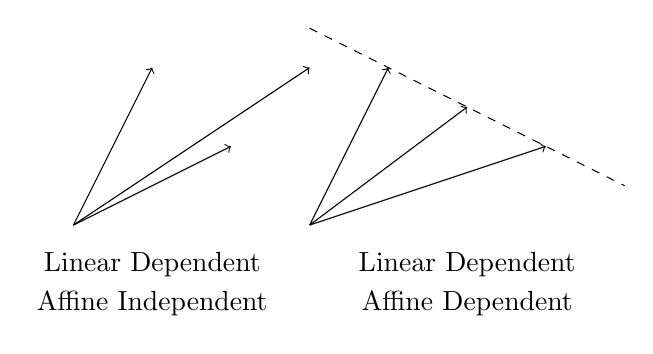
\begin{tikzpicture}
                        \draw [->] (1,1) -- (3,2);
                        \draw [->] (1,1) -- (4,3);
                        \draw [->] (1,1) -- (2,3);
                        \node at (2, 0.5) {Linear Dependent};
                        \node at (2, 0) {Affine Independent};
                        \draw [->] (4,1) -- (5,3);
                        \draw [->] (4,1) -- (6,2.5);
                        \draw [->] (4,1) -- (7,2);
                        \draw [dashed] (4,3.5) -- (8,1.5);
                        \node at (6, 0.5) {Linear Dependent};
                        \node at (6, 0) {Affine Dependent};
                    \end{tikzpicture}
                    \caption{Linearly Independent / Affinely Independent}
                \end{figure}

            \paragraph{Spanning set and basis}
                A collection of vectors $v^1, v^2, \dots, v^m$ of dimension $n$ is said to span $\mathcal{R}^n$ if any vector in $\mathcal{R}^n$ can be represented as a linear combination of $v^1, v^2, \dots, v^m$. $v^1, v^2, \dots, v^m$ is said to form a basis of $\mathcal{R}^n$ if the following conditions holds.
                \begin{itemize}
                    \item $v^1, v^2, \dots, v^m$ span $\mathcal{R}^n$.
                    \item If any of these vectors is deleted, the remaining collection of vector does not span $\mathcal{R}^n$.
                \end{itemize}

            \paragraph{Rank of a matrix}
                The span of the columns of a matrix $A$ is called the column space or the range, denoted $range(A)$. The span of the rows of a matrix $A$ is called the row space. The dimension of the column space and row space are equal, which is denoted by $rank(A)$. $rank(A) \le \min\{m,n\}$, if $rank(A) = \min\{m,n\}$, then $A$ is said to have full rank and $A$ is a basis of $\mathcal{R}^n$.

        \subsection{Polyhedral Sets}
            \paragraph{Convex sets}
                A set $S\subseteq \mathcal{R}^n$ is convex if $\forall x,y \in S, \lambda \in [0,1]$, we have $\lambda x + (1-\lambda)y \in S$

                \begin{figure}[!htp]
                    \centering
                    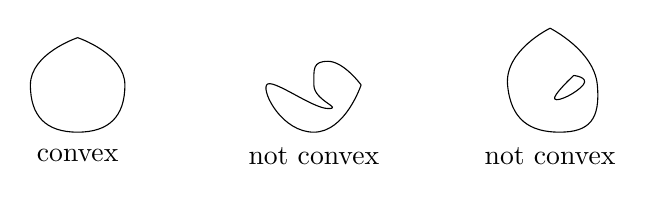
\begin{tikzpicture}[scale=0.6]
                        \draw plot [smooth, tension = 1.2] coordinates{(-5, 1) (-4, 0) (-5, -1) (-6, 0) (-5, 1)};
                        \draw plot [smooth, tension = 1.2] coordinates{(1, 0) (0.3, 0.5) (0, 0) (0.3, -0.5) (-1, 0) (0, -1) (1,0)};
                        \draw plot [smooth, tension = 1.2] coordinates{(5, 1.2) (4.1, 0) (5.2, -1) (6, 0) (5, 1.2)};
                        \draw plot [smooth, tension = 1.2] coordinates{(5.5, 0.2) (5.7, 0) (5.1, -0.3) (5.5, 0.2)};
                        \node at (0,-1.5) {not convex};
                        \node at (-5, -1.5) {convex};
                        \node at (5, -1.5) {not convex};
                    \end{tikzpicture}
                    \caption{A set is convex iff for any two points in the set, the line segment joining those two points lies entirely in the set}
                \end{figure}

                Let $x^1, ..., x^k \in \mathcal{R}^n$ and $\lambda \in \mathcal{R}^k$ be given such that $\lambda^Te=1$
                \begin{itemize}
                    \item The vector $\sum_{i=1}^k \lambda_i x ^i$ is said to be a convex combination of $x^1, ... , x^k$
                    \item The convex hull of $x^1, ... , x^k$ is the set of all convex combinations of these vectors, denoted $conv(x^1, ... ,x^k)$
                \end{itemize}

            \paragraph{Polyhedral, hyperplanes and half-spaces}
                \begin{itemize}
                    \item A polyhedron is a set of the form $\{x\in \mathcal{R}^n|Ax\le b\}=\{x \in \mathcal{R}^n | a^ix\le b^i, \forall i \in M\}$, where $A \in \mathcal{R}^{m\times n}$ and $b \in \mathcal{R}^m$
                    \item A polyhedron $P \subset \mathcal{R}^n$ is bounded if there exists a constant $K$ such that $|x_i|<K, \forall x \in P, \forall i \in [1, n]$, in this case the polyhedron is call polytope.
                    \item The lower-bound of $K$ is called diagonal denoted by $d$
                    \item A hyperplane is $\{x\in \mathcal{R}^n|a^Tx=b\}$
                    \item A half-space is $\{x\in \mathcal{R}^n|a^Tx\le b\}$
                \end{itemize}

            \paragraph{Open, close sets: boundary and interior}
                \begin{itemize}
                    \item Denote $N_\epsilon = \{y\in \mathcal{R}^n|\lVert y-x\rVert < \epsilon \}$ as the neighborhood of $x\in \mathcal{R}^n$
                    \item Given $S\subseteq \mathcal{R}^n$, x belongs to the interior of $S$, denoted by $int(S)$ if there is $\epsilon > 0$ such that $N_\epsilon(x) \le S$
                    \item $S$ is said to be an open set iff $S=int(S)$
                    \item $x$ belongs to the boundary $\partial S$ if $\forall \epsilon >0$, $N_\epsilon(x)$ contains at least one point in $S$ and a point not in $S$
                    \item $x\in S$ belongs to the closure of $S$, denoted $cl(s)$ if $\forall \epsilon > 0$, $N_\epsilon(x) \cap S = \emptyset$
                    \item $S$ is called closed iff $S=cl(S)$
                    \item In IP, LP, MIP, etc. we always work with close set. No \lq\lq{}$<$\rq\rq{} or \lq\lq{}$>$\rq\rq{}
                \end{itemize}

            \paragraph{Dimension of polyhedral}
                \begin{itemize}
                    \item A polyhedron $P$ is dimension $k$, denoted $dim(P)=k$, if the maximum number of affinely independent points in $P$ is $k+1$
                    \item A polyhedron $P\subseteq \mathcal{R}^n$ is full-dimensional if $dim(P) = n$
                    \item Let $M=\{1, 2, ..., m\}$, $M^= = \{i \in M | a_ix=b_i, \forall x \in P\}$, i.e. the equality set, $M^\le = M \setminus  M^=$, i.e. the inequality set. Then, Let $(A^=, b^=)$, $(A^\le, b^\le)$ be the corresponding rows of $(A, b)$, If $P\subseteq \mathcal{R}^n$, then $dim(P) = n - rank(A^=, b^=)$. To proof a constraint $(A^=, b^=)$ is an equality constraint, we need to proof all point in the closure of $P$ satisfied the constraint, to proof it is not an equality constraint, we need to find one point that is not in the hyperplane.
                    \item $x\in P$ is called an inner point of $P$ if $a^ix < b_i, \forall i \in M^\le$
                    \item $x\in P$ is called an interior point of $P$ if $a^ix < b_i, \forall i \in M$
                    \item Every nonempty polyhedron has at least one inner point
                    \item A polyhedron has an interior point iff $P$ is full-dimensional, i.e., there is no equality constraint
                \end{itemize}

        \subsection{E.P. and B.F.S.}
            \paragraph{Extreme point}
                A point $x$ in a convex set $X$ is called an extreme point iff $x$ cannot be represented as a strict convex combination of two distinct points of $X$. In other words, if $x = \lambda x_1 + (1 - \lambda) x_2$, then $x_1 = x_2 = x$.

                An alternative definition is as follows. Let the hyperplanes associated with the $(m + n)$ defining half-spaces of $X$ be referred to as defining hyperplanes of $X$. Furthermore, note that a set of defining hyperplanes are linearly independent if the coefficient matrix associated with this set of equations has full row rank. Then a point $x$ is said to be an extreme point if $x$ lies on some $n$ linearly independent defining hyperplanes of $X$. In addition, if more than $n$ defining hyperplanes pass through an extreme point, then such extreme point is called a degenerated extreme point.

            \paragraph{Basic feasible solution}
                Consider the system $\{A_{m\times n}x=b_m, x\ge 0\}$, suppose $rank(A, b) = rank(A) =m$, we can arrange $A$ and have a partition of $A$. Let $A=[B, N]$ where $B$ is $m\times m$ invertible matrix, and $N$ is a $m\times (n-m)$ matrix. The solution $x=\left[\begin{matrix}x_B\\x_N\end{matrix}\right]$ to the equation $Ax=b$, where
                \begin{equation}
                    x_B = B^{-1}b \nonumber
                \end{equation}
                and
                \begin{equation}
                    x_N = 0 \nonumber
                \end{equation}
                is called basic solution of system. If $x_B \ge 0$, it is called basic feasible solution. If $x_B > 0$ it is called non-degenerate basic feasible solution. For $x_B \ge 0$, if some $x_j = 0$, those components are called degenerated basic feasible solution. $B$ is called the basic matrix, $N$ is called nonbasic matrix.

            \paragraph{Correspondence between B.F.S and E.P.}
                \begin{theorem}
                    $x$ is an E.P. iff $x$ is a B.F.S.
                \end{theorem}
                
                \begin{proof}
                    ($\Rightarrow$) If $x$ is an extreme point, by definition, there are (at least) $n$ linearly independent defining hyperplanes at $x$, since $Ax = b$ provides $m$ linearly independent binding hyperplane, there must by some $p = n - m$ additional binding defining hyperplanes from the non-negativity constraints that together with $Ax = b$ provide $n$ linearly independent defining hyperplanes binding at $x$. Denoting these $p$ additional hyperplanes by $x_N = 0$, we therefore conclude that the system $Ax = b, x_N = 0$ has $x$ as the unique solution. Now, let $N$ represent the columns of the variables $x_N$ in $A$, and let $B$ be the remaining columns of $A$ with $x_B$ as the associated variables. Since $Ax = b$ can be written as $Bx_B + Nx_N = b$, this means that $B$ is $m \times m$ and invertible, and moreover, $x_B = B^{-1}b \ge 0$, since $x = (x_B, x_N)$ is a feasible solution. Therefore, $x$ is a basic feasible solution.

                    ($\Leftarrow$) If $x$ is a basic feasible solution, by definition, $x = (x_B, x_N)$ where correspondingly $A = (B, N)$ such that $x_B = B^{-1}b \ge 0$ and $x_N = 0$. This means that the $n$ hyperplanes $Ax = b, x_N = 0$ are binding at $x$ and are linearly independent. Thus, $x$ is an extreme point.
                \end{proof}

    \section{Simplex Method}
        \subsection{Search Algorithm}
            \paragraph{Improving search algorithm}
                A simplex method is a search algorithm, for each iteration it finds a not-worse solution, which can be represented as
                \begin{equation}
                    x^t = x^{t-1}+\lambda_{t-1}d^{t-1} \nonumber 
                \end{equation}
                Where $x^t$ is the solution of the $t$th iteration, $\lambda_t$ is the step length of $t$th iteration, and $d^t$ is the direction of the $t$th iteration.
                    
            \paragraph{Optimality test}
                \begin{align}
                    z &= cx \nonumber\\
                    & = \left[\begin{matrix}c_B & c_N\end{matrix} \right] \left [ \begin{matrix}x_B \\ x_N \end{matrix} \right] \nonumber \\
                    & = c_B x_B + c_N x_N \nonumber \\
                \text{and } \quad& Ax=b \nonumber \\
                    \Rightarrow & Bx_B + Nx_N = b, x_B\ge 0, x_N\ge 0\nonumber \\
                    \Rightarrow & x_B = B^{-1}b-B^{-1}Nx_N\nonumber \\
                    \Rightarrow & z = c_BB^{-1}b-c_BB^{-1}Nx_N+c_Nx_N\nonumber
                \end{align}
                for current solution $\hat{x}=\left [\begin{matrix}\hat{x_B} \\ 0\end{matrix}\right]$, $\hat{z} = c_BB^{-1}b$, then
                \begin{equation}
                    z - \hat{z} = \left[\begin{matrix}0 & c_N - c_BB^{-1}N \end{matrix} \right] \left[ \begin{matrix}x_B \\ x_N \end{matrix}\right] \nonumber
                \end{equation}
                The $c_N - c_BB^{-1}N$ is the reduced cost, for a minimized problem, if $c_N - c_BB^{-1}N > 0$ means $z - \hat{z} \ge 0$, it reaches the optimality because we cannot find a solution less than $\hat{z}$.
                            
            \paragraph{Find direction}
                Suppose we choose $x_k$ as a candidate to pivot into Basis\\
                \begin{equation}
                    x = \left[ \begin{matrix}B^{-1}b-B^{-1}a_kx_k \\ 0+e_kx_k\end{matrix}\right]=\left[ \begin{matrix}B^{-1}b \\ 0\end{matrix} \right] + \left[ \begin{matrix} -B^{-1}a_k \\ e_k \end{matrix} \right]x_k \nonumber
                \end{equation}
                In this form, we can see: $x$ is the result after $t$th iteration, $\left[ \begin{matrix}B^{-1}b \\ 0\end{matrix} \right]$ is the result after $(t-1)$th iteration. $ \left[ \begin{matrix} -B^{-1}a_k \\ e_k \end{matrix} \right]$ is the iteration direction, $x_k$ is the step length. The only requirement of $x_k$ is $r_k < 0$ where $r_k=c_k - z_k$ is reduce cost, which is the $k$th entry of $c_N - c_BB^{-1}N$. Generally speaking, we usually take $r_k = \min\{c_j - z_j\}$ (which in fact can not guarantee the efficient of the algorithm.)

            \paragraph{Find the step length}
                We need to guarantee the non-negativity, so for each iteration, we need to make sure $x\ge 0$. Which means
                \begin{equation}
                    B^{-1}b-B^{-1}a_kx_k \ge 0 \nonumber 
                \end{equation}
                Denote $B^{-1}b$ as $\bar{b}$, denote $B^{-1}a_k$ as $y_k$. If $y_k \le 0$, we can have $x_k$ as large as infinite, which means unboundness. If $y_k > 0$ now we can use the minimum ratio to guarantee non-negativity.
                \begin{equation}
                    \forall i \in B, \bar{b}_i - y_{ik} x_k \ge 0 \Rightarrow x_k = \min_{i \in B} \{\frac{\bar{b}_i}{y_{ik}}, y_{ik} > 0\}.\nonumber
                \end{equation}

        \subsection{Find Initial Solution}
            \paragraph{Non-trivial case}
                If some of the constraint is not in $\sum_{i=1}^na_ix_i \le 0$ form, we cannot add a positive slack variable. In this case, we add an artificial variable other than slack variable.
                \begin{equation}
                    \sum_{i=1}^n a_ix_i \ge (or =) 0 \Rightarrow \sum_{j=1}^n a_ix_i + x_a = 0 \nonumber
                \end{equation}
                Notice that in an optimal solution, $x_a = 0$, otherwise it is not valid.\\
                Artificial variables are only a tool to get the simplex method started. A so-called Two-phase Method is describe in this section.
            
            \paragraph{Two-Phase method}
                \begin{itemize}
                    \item Phase I: Solve the following program start with a basic feasible solution $x=0, x_a=b$, i.e., the artificial variable forms the basis.
                    \begin{align}
                        \min \quad & 1x_a \nonumber\\
                        \text{s.t.} \quad & Ax + x_a = b \nonumber\\
                                          & x \ge 0 \nonumber\\
                                          & x_a \ge 0 \nonumber
                    \end{align}
                    If the optimal $1x_a \ne 0$, infeasible, stop. Otherwise proceed Phase II.
                    \item Phase II: Remove the columns of artificial variables, replace the objective function with the original objective function, proceed to solve simplex method.
                \end{itemize}               
                
            \paragraph{Discussion}
                \begin{itemize}
                    \item Case A: $x_a \ne 0$. Infeasible.
                    \item Case B.1: $x_a = 0$ and all artificial variables are out of the basis. At the end of Phase I, we derive
                    \begin{align}
                        \begin{tabular} {|c|c|c|c|c|}
                            \hline
                            $x_0$ & $x_B$ & $x_N$ & $x_a$ & RHS \\
                            \hline
                            1 & 0 & 0 & -1 & 0\\
                            \hline
                            0 & $I$ & $B^{-1}N$ & $B^{-1}$ & $B^{-1}b$ \\
                            \hline
                        \end{tabular} \nonumber
                    \end{align}
                    We can discard $x_a$ columns, (or we can leave it because it keeps track of $B^{-1}$), and then we do the Phase II
                    \begin{align}
                        \begin{tabular} {|c|c|c|c|}
                            \hline
                            $z$ & $x_B$ & $x_N$ & $RHS$ \\
                            \hline
                            1 & 0 & $c_BB^{-1}N - c_N$ & $c_BB^{-1}b$ \\
                            \hline
                            0 & $I$ & $B^{-1}N$ & $B^{-1}b$ \\
                            \hline
                        \end{tabular} \nonumber     
                    \end{align}
                    \item Case B.2: Some artificial variables are in the basis at zero values. This is because of degeneracy. We pivot on those artificial variables, once they leave the basis, eliminate them.
                \end{itemize}

        \subsection{Degeneracy and Cycling}
            \paragraph{Degeneracy}
                If the basic variable $x_B$ is not strictly $> 0$, i.e. if some basic variable equals to 0, we call it degenerate.

            \paragraph{Cycling}
                In the degenerate case, pivoting by the simplex rule does not always give a strict decrease in the objective function value, because it may have $b_r = 0$. It is possible that the tableau may repeat if we use the simplex rule.Geometrically speaking, it means that at the same point - extreme point - it corresponds to more than one feasible solutions, so when we are pivoting, we stays at the same place. However, in computer algorithm, we rarely care about cycling because the data in computer is not precise, it is very hard to get into cycling.

            \paragraph{Cycling prevent}
                \begin{itemize}
                    \item Lexicographic rule
                    \begin{itemize}
                        \item For entering variable, same as simplex rule
                        \item For leaving variable, if there is a tie, choose the variable with the smallest $\frac{y_{r1}}{y_{rk}}$.
                    \end{itemize}
                    \item Bland's rule
                    \begin{itemize}
                        \item For entering variable, choose the variable with smallest index where $z_j - c_j \le 0$
                        \item For leaving variable, if there is a tie, choose the variable with smallest index.
                    \end{itemize}
                    \item Successive ratio rule
                    \begin{itemize}
                        \item Select the pivot column as any column $k$ where $z_k - c_k \le 0$
                        \item Given $k$, select the pivot row $r$ as the minimum successive ratio row associated with column $k$. In other words, for pivot columns where there is no tie in the usual minimum ratio, the successive ratio rule reduces to the simplex rule.
                    \end{itemize}
                \end{itemize}

    \section{Revised Simplex Method}
        \subsection{Key to Revised Simplex Method}
            The procedure of Simplex Method is (almost) exactly the same as original simplex method. However, notice that we don't need to use $N$ so for the revised simplex method, we don't calculate any matrix related to $N$

            The original matrix:

            \begin{align}
                \begin{tabular} {|c|c|c|c|}
                    \hline
                    $z$ & $x_B$ & $x_N$ & $RHS$ \\
                    \hline
                    1 & 0 & $c_BB^{-1}N - c_N$ & $c_BB^{-1}b$ \\
                    \hline
                    0 & $I$ & $B^{-1}N$ & $B^{-1}b$ \\
                    \hline
                \end{tabular} \nonumber     
            \end{align}

            The revised matrix:

            \begin{align}
                \begin{tabular} {|c|c|}
                    \hline
                    Basic Inverse & RHS \\
                    \hline
                    $w=c_BB^{-1}$ & $c_B\bar{b} = c_BB^{-1}b$\\
                    \hline
                    $B^{-1}$ & $\bar{b} = B^{-1}b$\\
                    \hline
                \end{tabular} \nonumber
            \end{align}

            For each pivot iteration, calculate $z_j - c_j = wa_j - c_j = c_BB^{-1}a_j - c_j, \forall j\in N$, pivot rules are the same as simplex method, each time find a variable $x_k$ to enter basis

            \begin{align}
                \begin{tabular}{|c|c|c|c|}
                    \cline{1-2} \cline{4-4} $B^{-1}$ & RHS & & $x_k$ \\
                    \cline{1-2} \cline{4-4} $w$ & $c_B\bar{b}$ & & $z_k-c_k$ \\
                    \cline{1-2} \cline{4-4} $B^{-1}$ & $\bar{b}$ & & $y_k$ \\
                    \cline{1-2} \cline{4-4}
                \end{tabular} \nonumber
            \end{align}

            Do the minimum ratio rule to find the variable $x_r$ to leave the basis

            \begin{align}
                \begin{tabular}{|c|c|c|c|}  
                    \cline{1-2} \cline{4-4} $B^{-1}$ & RHS & & $x_k$ \\
                    \cline{1-2} \cline{4-4} $w$ & $c_B\bar{b}$ & & $z_k-c_k$ \\
                    \cline{1-2} \cline{4-4} & $\bar{b}_1$ & & $y_{1k}$\\
                    & $\bar{b_2}$ & & $y_{2k}$\\
                    & $\cdots$ & & $\cdots$\\
                    $B^{-1}$ & $\bar{b}_r$ & & $y_{rk}$(pivot at here)\\
                    & $\cdots$ & & $\cdots$\\
                    & $\bar{b}_m$ & & $y_{mk}$\\
                    \cline{1-2} \cline{4-4} 
                \end{tabular} \nonumber
            \end{align}

        \subsection{Comparison between Simplex and Revised Simplex}
            \paragraph{Advantage of revised simplex}
                \begin{itemize}
                    \item Save storage memory
                    \item Don\rq{}t need to calculate N (including $B^{-1}N$ and $c_BB^{-1}N$)
                    \item More accurate because round up errors will not be accumulated 
                \end{itemize}

            \paragraph{Disadvantage of revised simplex}
                Need to calculate $wa_j$ for all $j \in N$ (in fact don\rq{}t need to calculated it for the variable just left the basis) 

            \paragraph{Computation complexity}
                \begin{align}
                    \begin{tabular}{|c|c|c|}
                        \hline Method & Type & Operations\\
                        \hline Simplex & $\times$ & $(m+1)(n-m+1)$\\
                        \cline{2-3} & $+$ & $m(n-m+1)$\\
                        \hline Revised Simplex & $\times$ & $(m+1)^2+m(n-m)$ \\
                        \cline{2-3} & $+$ & $m(m+1)+m(n-m)$ \\
                        \hline
                    \end{tabular} \nonumber
                \end{align}

            \paragraph{When to use?}
                \begin{itemize}
                    \item When $m >> n$, do revise simplex method on the dual problem
                    \item When $m \simeq n$, revise simplex method is not as good as simplex method
                    \item When $m << n$ perfect for revise simplex method.
                \end{itemize}
                        
        \subsection{Decomposition of B inverse}
            Let $B=\{ a_{B_1}, a_{B_2}, ..., a_{B_r}, ..., a_{B_m}\}$ and $B^{-1}$ is known.
            If $a_{B_r}$ is replaced by $a_{B_k}$, then $B$ becomes $\bar{B}$. Which means $a_{B_r}$ enters the basis and $a_{B_k}$ leaves the basis. \\
            Then $\bar{B}^{-1}$ can be represent by $B^{-1}$. Noting that $a_k=By_k$ and $a_{B_i}=Be_i$, then
            \begin{align}
                \bar{B} & = (a_{B_1}, a_{B_2}, ...,a_{B_{r-1}}, a_k, a_{B_{r+1}}, a_m) \nonumber \\
                & = (Be_1, Be_2, ..., Be_{r-1}, By_k, Be_{r+1}, ..., Be_m) \nonumber \\
                & = BT \nonumber
            \end{align}
            where $T$ is
            \begin{equation}
                T=\left[ \begin{array}{cccccccc}
                    1 & 0 & ... & 0 & y_{1k} & 0 & ... & 0 \\
                    0 & 1 & ... & 0 &  y_{2k} & 0 & ... & 0 \\
                    \vdots & \vdots & & \vdots & \vdots & \vdots & & \vdots \\
                    0 & 0 & ... & 1 & y_{r-1,k} & 0 & ... & 0 \\
                    0 & 0 & ... & 0 & y_{rk} & 0 & ... & 0 \\
                    0 & 0 & ... & 0 &  y_{r+1,k} & 1 & ... & 0 \\
                    \vdots & \vdots & & \vdots & \vdots & \vdots & & \vdots \\
                    0 & 0 & ... & 0 &  y_{mk}& 0 & ... & 1 \\
                \end{array} \right] \nonumber
            \end{equation}
            and 
            \begin{equation}
                E =  T ^{-1}=\left[ \begin{array}{cccccccc}
                    1 & 0 & ... & 0 & \frac{-y_{1k}}{y_{rk}} & 0 & ... & 0 \\
                    0 & 1 & ... & 0 & \frac{-y_{2k}}{y_{rk}} & 0 & ... & 0 \\
                    \vdots & \vdots & & \vdots & \vdots & \vdots & & \vdots \\
                    0 & 0 & ... & 1 & \frac{-y_{r-1,k}}{y_{rk}} & 0 & ... & 0 \\
                    0 & 0 & ... & 0 & \frac{1}{y_{rk}} & 0 & ... & 0 \\
                    0 & 0 & ... & 0 & \frac{-y_{r+1,k}}{y_{rk}} & 1 & ... & 0 \\
                    \vdots & \vdots & & \vdots & \vdots & \vdots & & \vdots \\
                    0 & 0 & ... & 0 &  \frac{-y_{mk}}{y_{rk}} & 0 & ... & 1 \\
                \end{array} \right] \nonumber
            \end{equation}
            For each iteration, i.e. one variable enters the basis and one leaves the basis, $\bar{B}^{-1}=T^{-1}B^{-1}=EB^{-1}$. Given that the first iteration starts from slack variables, the first basis $B_1$ is $I$, then we have
            \begin{equation}
                B^{-1}_t=E_{t-1} E_{t-2} \cdots E_{2} E_{1} I\nonumber
            \end{equation}
            Using $E$ in calculation can simplify the product of matrix where
            \begin{align}
                cE &= {c_1,c_2,...,c_m} \left[ \begin{array}{cccccc}
                1 & 0 & ... & g_1 & ... & 0 \\
                0 & 1 & ... & g_2 & ... & 0 \\
                \vdots & \vdots & & \vdots & & \vdots \\
                0 & 0 & ... & g_m & ... & 1 \\
                \end{array} \right] \nonumber \\
                &= (c_1, c_2, ... ,c_{r-1}, cg, c_{r+1}, ..., c_m) \nonumber
            \end{align}
            and
            \begin{align}
                Ea &=  \left[ \begin{array}{cccccc}
                1 & 0 & ... & g_1 & ... & 0 \\
                0 & 1 & ... & g_2 & ... & 0 \\
                \vdots & \vdots & & \vdots & & \vdots \\
                0 & 0 & ... & g_m & ... & 1 \\
                \end{array} \right]
                 \left[ \begin{array}{c}
                a_1 \\
                a_2 \\
                \vdots \\
                a_m \\
                \end{array} \right] \nonumber \\
                &= 
                \left[ \begin{array}{c}
                a_1 \\
                a_2 \\
                \vdots \\
                a_{r-1} \\
                0 \\
                a_{r+1} \\
                \vdots \\
                a_m \\
                \end{array} \right] +
                a_r\left[ \begin{array}{c}
                g_1 \\
                g_2 \\
                \vdots \\
                g_{r-1} \\
                g_r \\
                g_{r+1} \\
                \vdots \\
                g_m \\
                \end{array} \right] \nonumber \\
                &=\bar{a}+a_rg \nonumber
            \end{align}
            Then we can calculate $w$, $y_k$ and $\bar{b}$
            \begin{align}
                w&=c_BB^{-1} = c_BE_{t-1}E_{t-2}...E_2E_1 \nonumber \\
                y_k &=B^{-1}a_k = E_{t-1}E_{t-2}...E_2E_1a_k \nonumber \\
                \bar{b}&=B^{-1}_{t+1}b=E_tE_{t-1}E_{t-2}...E_2E_1b \nonumber
            \end{align}

    \section{Duality}
        \subsection{Dual Formulation}
            For any prime problem
            \begin{align}
                \text{min} \quad & cx \nonumber\\
                \text{s.t.} \quad & Ax\ge b \nonumber\\
                            & x\ge 0 \nonumber
            \end{align}
            we can have a dual problem
            \begin{align}
                \text{max} \quad & wb \nonumber \\
                \text{s.t.} \quad & wA\le c\nonumber\\
                            & w \ge 0\nonumber
            \end{align}
            
        \subsection{Mixed Forms of Duality}
            For the following prime problem
            \begin{align}
                \text{P(or D)} \quad \min \quad & c_1x_1 + c_2x_2 + c_3x_3 \nonumber\\
                \quad \text{s.t.} \quad & A_{11}x_1 + A_{12}x_2 + A_{13}x_3 \ge b_1 \nonumber\\
                                        & A_{21}x_1 + A_{22}x_2 + A_{23}x_3 \le b_2 \nonumber\\
                                        & A_{31}x_1 + A_{32}x_2 + A_{33}x_3 = b_3 \nonumber\\
                                        & x_1 \ge 0 \nonumber\\
                                        & x_2 \le 0 \nonumber\\
                                        & x_3 \quad \text{unrestricted} \nonumber
            \end{align}
            The dual of the problem
            \begin{align}
                \text{D(or P)} \quad \max \quad & w_1b_1 + w_2b_2 + w_3b——3 \nonumber\\
                \quad \text{s.t.} \quad & w_1A_{11} + w_2A_{21} + w_3A_{31} \le c_1 \nonumber\\
                                        & w_1A_{12} + w_2A_{22} + w_3A_{32} \ge c_2 \nonumber\\
                                        & w_1A_{13} + w_2A_{23} + w_3A_{33} = c_3 \nonumber\\
                                        & w_1 \ge 0 \nonumber\\
                                        & w_2 \le 0 \nonumber\\
                                        & w_3 \quad \text{unrestricted} \nonumber
            \end{align}
            In sum, the relation between primal and dual problems are listed as following\\
            \begin{table}[!htp]
                \centering
                \begin{tabular}{|c|c|c|c|c|}
                    \hline & Minimization& & Maximization& \\
                    \hline & $\geq 0$ & $\longleftrightarrow$ & $\leq 0$ & \\
                    Var & $\leq 0$ & $\longleftrightarrow$ & $\geq 0$ & Cons \\
                    & Unrestricted & $\longleftrightarrow$ & = & \\
                    \hline & $\geq 0$ & $\longleftrightarrow$ & $\geq 0$ & \\
                    Cons & $\leq 0$ & $\longleftrightarrow$ & $\leq 0$ & Var \\
                    & = & $\longleftrightarrow$ & Unrestricted & \\
                    \hline
                \end{tabular}
            \end{table}                

        \subsection{Primal-Dual Relationships}
            \paragraph{Weak duality property}
                Let $x_0$ be any feasible solution of a primal minimization problem,
                \begin{equation}
                    Ax_0 \ge b, \quad x_0\ge 0 \nonumber
                \end{equation}
                Let $x_0$ be any feasible solution of a dual maximization problem,
                \begin{equation}
                    w_0A \le c, \quad w_0\ge 0 \nonumber
                \end{equation}
                Therefore, we have
                \begin{equation}
                    cx_0 \ge w_0Ax_0 \ge w_0b \nonumber
                \end{equation}
                which is called the weak duality property. This property is for any feasible solution in the primal and dual problem.\\
                Therefore, any feasible solution in the maximization problem gives the lower bound of its dual problem, which is a minimization problem, vice versa. We use this to give the bounds in using linear relaxation to solve IP problem.

            \paragraph{Fundamental theorem of duality}
                With regard to the primal and dual LP problems, one and only one of the following can be true. 

                \begin{itemize}
                    \item Both primal and dual has optimal solution $x^*$ and $w^*$, where $cx^* = w^*b$
                    \item One problem has an unbounded optimal objective value, the other problem must be infeasible
                    \item Both problems are infeasible.
                \end{itemize}

                \begin{table}[!htp]
                    \centering
                    \begin{tabular}{|c|c|c|}
                        \hline P & & D \\
                        \hline Optimal & $\Rightarrow$ & Optimal \\
                        Degeneracy & & Multiple optimal \\
                        (or Multiple optimal) & & (or Degeneracy) \\
                        \hline Infeasible & $\Rightarrow$ & Unbounded or Infeasible \\
                        \hline Unbounded & $\Rightarrow$ & Infeasible \\
                        \hline
                    \end{tabular}
                \end{table}

            \paragraph{Strong duality property}
                From KKT condition, we know that in order to make $x^*$ the optimal solution, the following condition should be met.
                \begin{itemize}
                    \item Primal Optimal: $Ax^* \ge b$, $x^*\ge 0$
                    \item Dual Optimal: $w^*A \le c$, $w^*\ge 0$
                    \item Complementary Slackness:
                \begin{equation}
                    \begin{cases}
                        w^*(Ax^*-b) = 0\\
                        (c-w^*A)x^* = 0
                    \end{cases} \nonumber
                \end{equation}
                \end{itemize}
                The first condition means the primal has an optimal solution, the second condition means the dual has an optimal solution. The third condition means $cx^*=w^*b$, which is also called strong duality property.

            \paragraph{Complementary slackness theorem}
                Let $\bm{x^*}$ and $\bm{w^*}$ be any feasible solutions, they are optimal iff
                \begin{align}
                    (c_j - \bm{w^*}\bm{a_j})x_j^* &= 0, \quad j = 1,...,n\nonumber \\
                    w_i^*(\bm{a^i}\bm{x^*} - b_i) &= 0, \quad i = 1,...,m\nonumber
                \end{align}
                In particular
                \begin{align}
                    x_j^*>0 &\Rightarrow \bm{w^*}\bm{a_j} = c_j \nonumber \\
                    \bm{w^*}\bm{a_j} < c_j &\Rightarrow x_j^* = 0 \nonumber \\
                    w_i^* >0 &\Rightarrow \bm{a^i}\bm{x^*} = b_i \nonumber \\
                    \bm{a^i}\bm{x^*} > b_i &\Rightarrow w_i^*=0\nonumber
                \end{align}
                It means, if in optimal solution a variable is positive (has to be in the basis), the correspond constraint in the other problem is tight. If the constraint in one problem is not tight, the correspond variable in the other problem is zero.

            \paragraph{Use dual to solve the primal}
                in the dual problem, we solved some $w$ which is positive, we can know that the correspond constraint in primal is tight, furthermore we can solve the basic variables from those tight constraints, which becomes equality and we can solve it using Gaussian-Elimination.

        \subsection{Shadow Price}
            \paragraph{Shadow price under non-degeneracy}
                Let $B$ be an optimal basis for primal problem and the optimal solution $x^*$ is non-degenerated.
                \begin{equation}
                    z=c_BB^{-1}b - \sum_{j\in N}(z_j - c_j)x_j = w^*b - \sum_{j\in N}(z_j - c_j)x_j \nonumber
                \end{equation}
                therefore
                \begin{equation}
                    \frac{\partial z^*}{\partial b_i} = c_BB^{-1}_i = w_i^* \nonumber
                \end{equation}
                $w^*$ is the shadow prices for the right-hand-side vectors. We can also regard it as the incremental cost of producing one more unit of the $i$th product. Or $w^*$ is the fair price we would pay to have an extra unit of the $i$th product.

            \paragraph{Shadow price under degeneracy}
                For shadow price under degeneracy, the $w^*$ may not be the true shadow price, for it may not be the right basis. In this case, the partial differentiation may not be valid, for component $b_i$, if $x_i = 0$ and $x_i$ is a basic variable, we can't find the differentiation.

        \subsection{Dual Simplex Method}
            Occasionally, an initial feasible solution for the Simplex Method might be difficult to acquired, for example, when $\mathbf{0}$ is not an initial solution, or, in some other cases, a basic infeasible solution is known in advance. To solve the LP, we can take advantage of the LP Strong Duality Theorem, and solve the dual problem to optimality instead of the prime problem. Such technique is called the Dual Simplex Method. The details of such method is as follows (for minimization problems)

            \begin{enumerate}
                \item Choose an initial basic solution $x_B$ and corresponding basis matrix $B$ so that $c_BB^{-1}A_j - c_j \ge 0$ for all $j \in J$, where $J$ is the set of non-basic variables.
                \item Construct a simplex tableau using this initial solution.
                \item If $\bar{b} = B^{-1}b \ge 0$, then an optimal solution has been achieved; STOP. Otherwise, the dual problem is feasible, GOTO STEP 4.
                \item Choose a leaving variable $x_{B_i} = \bar{b}_i$ so that $\bar{b}_i < 0$
                \item Choose the index of the entering variable $x_j$ using the following minimum ratio test:
                \begin{equation*}
                    \frac{z_j - c_j}{\bar{a}_{j_i}} = \min \{\frac{z_k - c_k}{\bar{a}_{k_i}}|k \in J, \bar{a}_{j_i} < 0\}
                \end{equation*}
                \item If no entering variable can be selected ($\bar{a}_{j_i} \ge 0, \forall k \in K$) then the dual problem is unbounded and the prime problem is infeasible. STOP
                \item Using a standard simplex pivot, on element $\bar{a}_{j_i}$, thus causing $w_{B_i}$ to become 0 (and thus feasible) and causing $x_j$ to enter the basis. GOTO STEP 3.
            \end{enumerate}

            In general, the Dual Simplex Method is (almost) the same as a Simplex Method. The Dual Simplex Method starts with an infeasible basic solution, during each iteration, it maintains dual feasibility and work towards primal feasibility. In Dual Simplex Method, the old Right Hand Side becomes new $z_j - c_j$, and the old $z_j - c_j$ become new Right Hand Side.

    % \bibliography{literature}
\end{document}